%!TEX root=main.tex
\subsection{Skip Connection}
\label{sec:skip_conn}

Skip connection, as the other of the most important techniques to enable training deep networks, also has significant effect to the loss landscape. 

As mentioned in \cite{li2018visualizing}, the skip connections are able to bring smoother loss surface after training. 

\begin{figure}[htp]
	\label{fig:skip_conn_final}
	\begin{tabular}{cc}
		\subfloat[With Skip Connection]{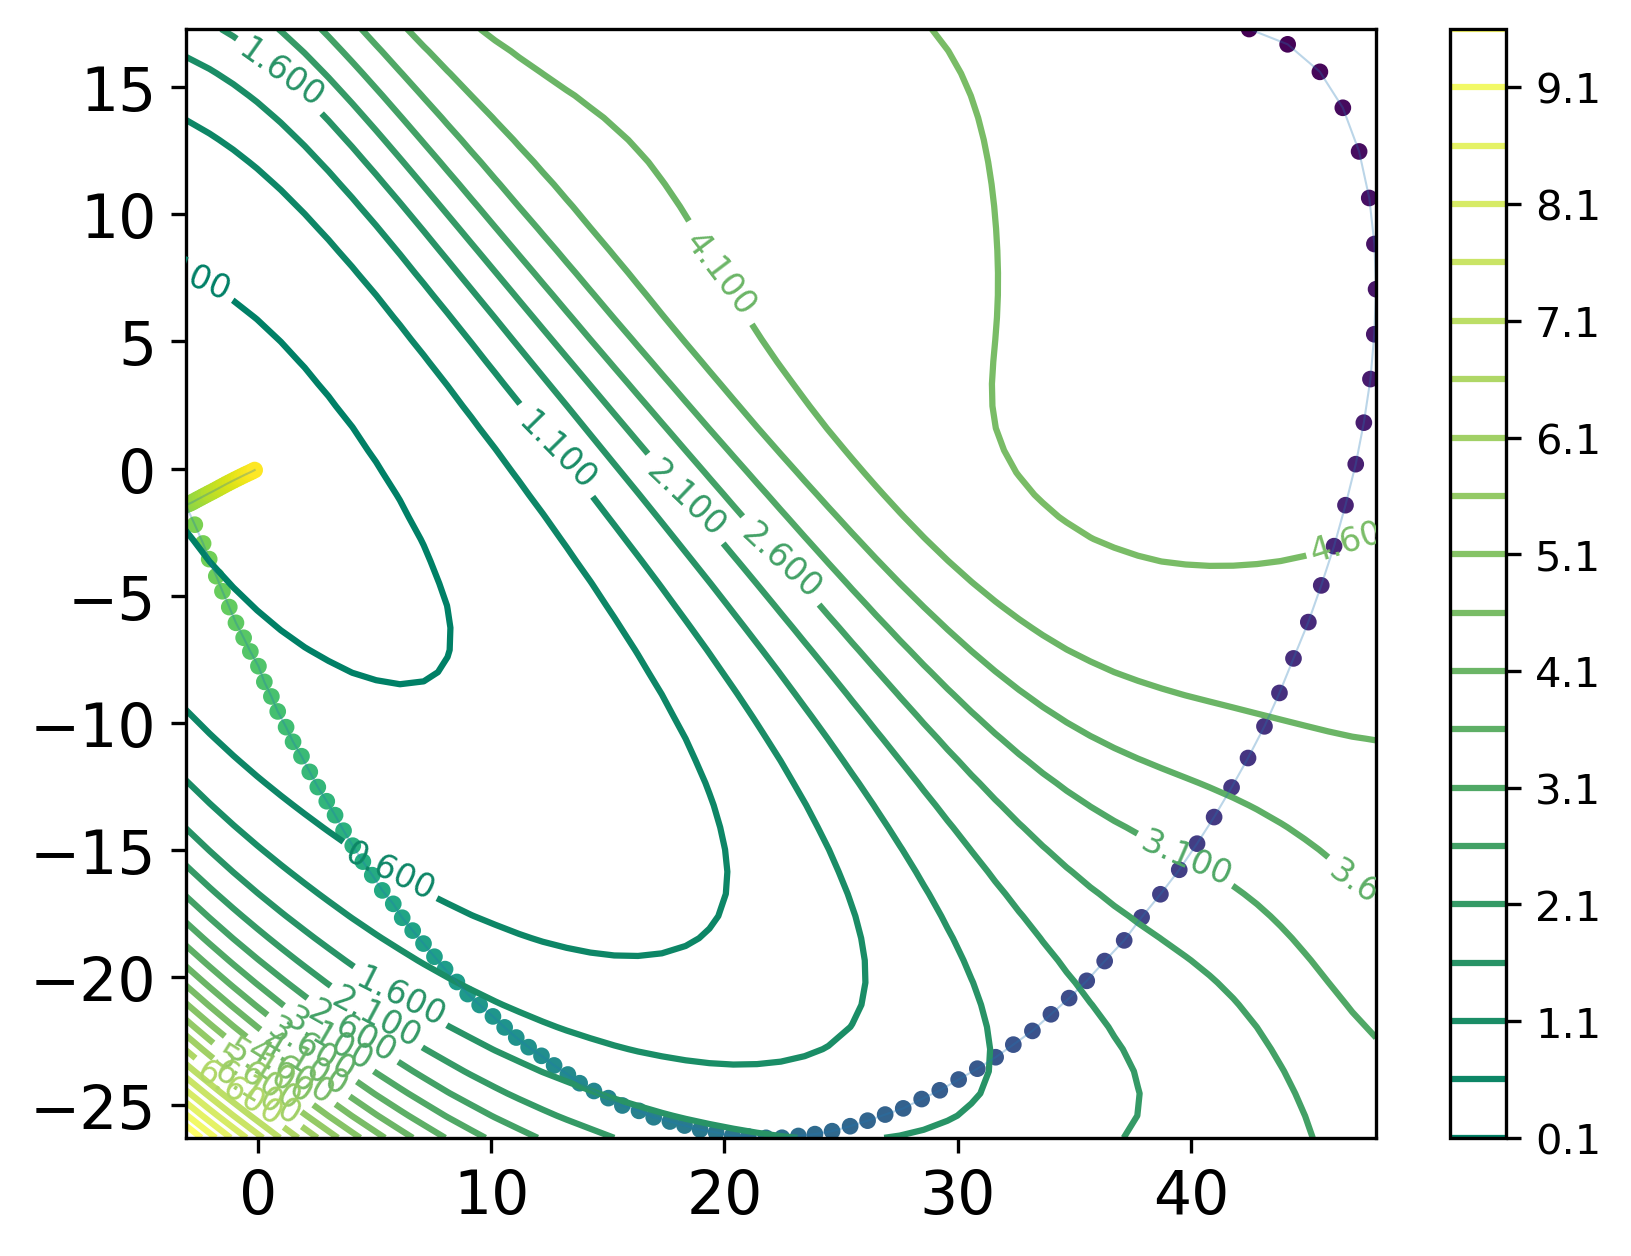
\includegraphics[width =  0.45\linewidth]{results/skip_conn/resnet20_with_final.png}} &
		\subfloat[Without Skip Connection]{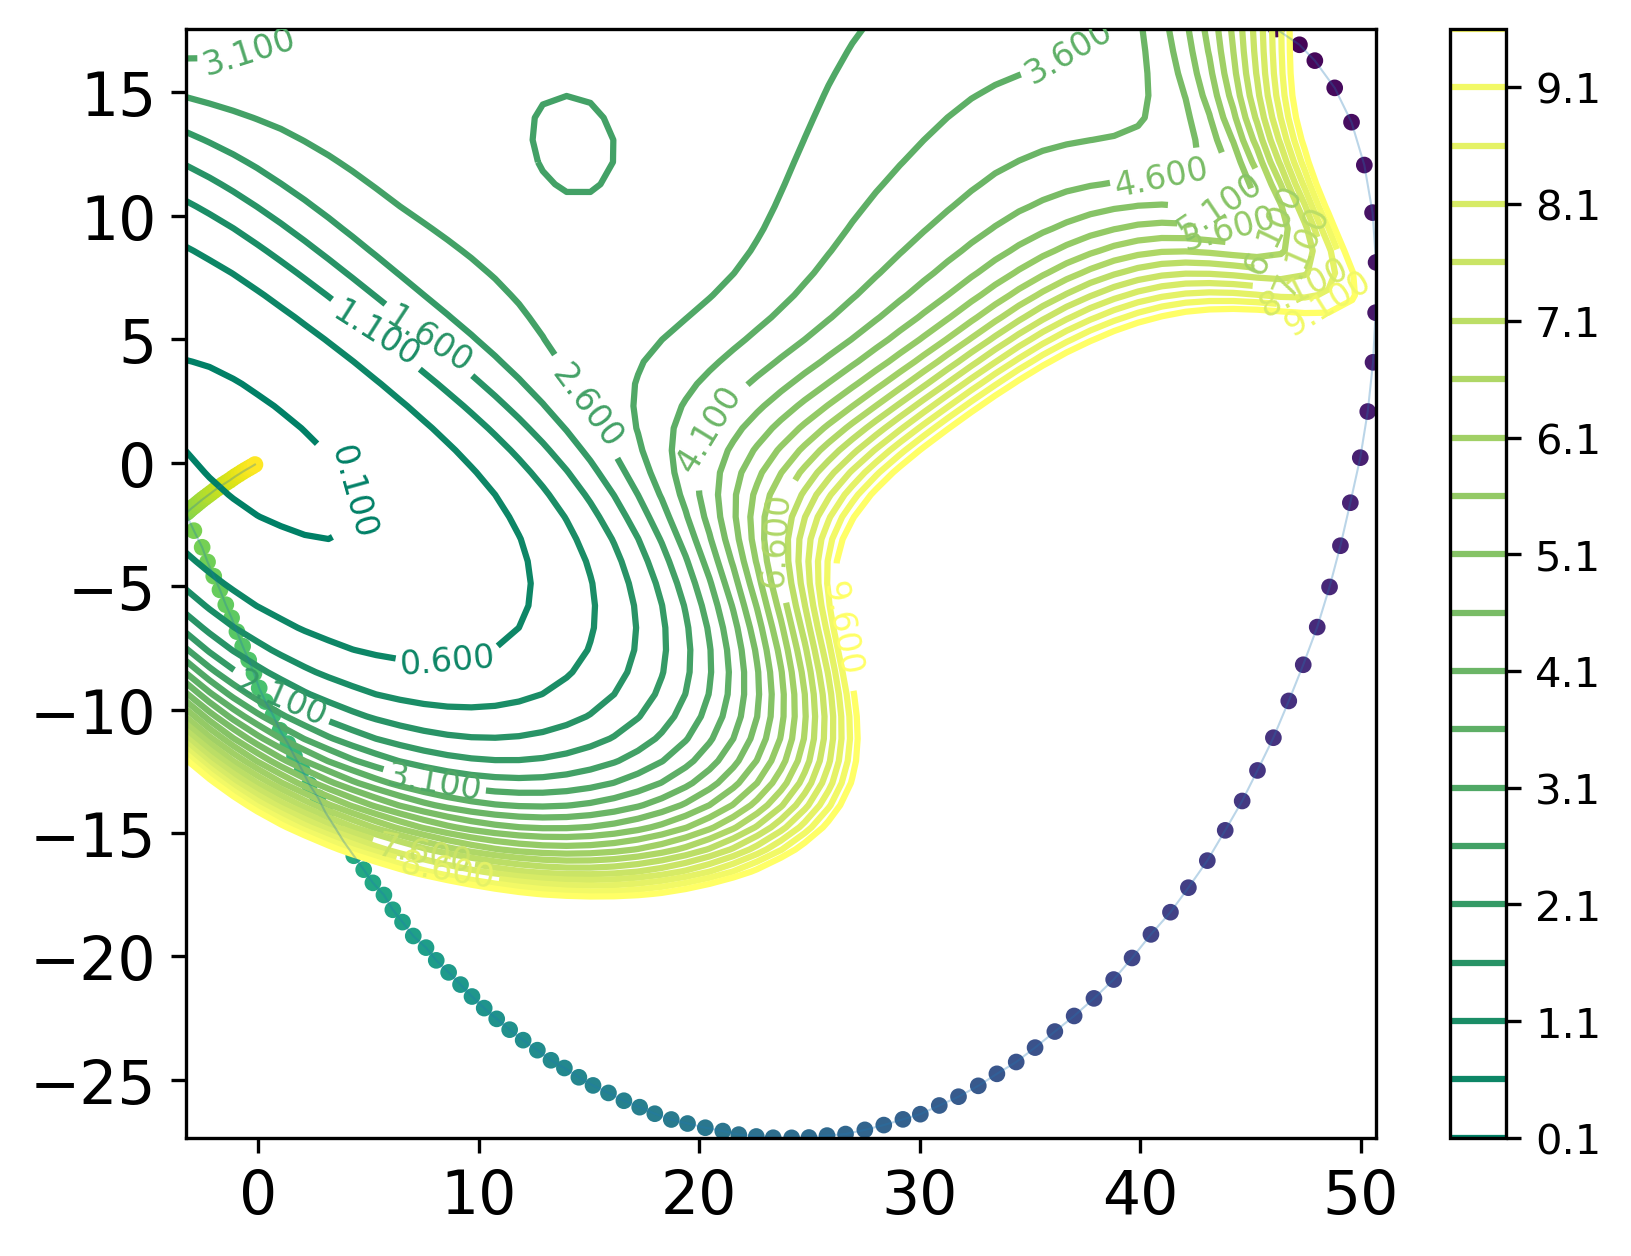
\includegraphics[width =  0.45\linewidth]{results/skip_conn/resnet20_without_final.png}} 
	\end{tabular}
	\caption{Loss landscape with/without Skip Connection (Trained)}
\end{figure}

%However, how does the landscape look at the initialization for these architectures?
Then, a natural question arise: would the skip connections ensure the smoother loss surface even prior to training? 
To this end, we picture the loss landscapes for the initialized weights with the same directions for projection in . 



